\chapter{Níveis e Compensações}\label{chap:10:niveis_compensacoes}

O sistema de nivelamento amador utilizado no Go funciona da seguinte maneira. Jogadores iniciantes recebem automaticamente o nível de 35 kyu e, conforme aprendem técnicas básicas do jogo, eles rapidamente avançam a escada kyu até chegar a algo entre, aproximadamente 20 a 10 kyu. Essa melhora rápida presume, claro, que se estude e se jogue algumas vezes na semana por alguns meses. De 10 a 1 kyu, o progresso é usualmente muito mais devagar. Assim que um jogador amador se torna um expert, ele recebe o nível de 1 dan (\emph{shodan} em japonês), ou de uma organização ou por simplesmente medir sua força contra outros jogadores de força dan. Níveis amadores dan vão até 7 dan em geral. Níveis profissionais vão de 1 a 9 dan, mas eles estão em uma escala diferente, portanto não possuem nenhum nível correspondente em níveis amadores. Um profissional 1 dan deveria estar apto a dar perto de três pedras de compensação a um amador de nível 5 dan, e ainda ter pelo menos 50\% de chance de vitória. O sistema de compensação no Go oferece ao jogador mais fraco uma chance realística de vitória quando se joga com alguém mais forte, dado que a compensação esteja correta, claro.

Jogadores de força igual geralmente utilizam um método chamado de \emph{nigiri} para determinar quem tomará branco ou preto. Quando o nigiri é utilizado, um dos jogadores toma uma quantidade arbitrária de pedras brancas enquanto que o jogador preto escolhe uma ou duas pedras, essencialmente uma variante do jogo de par-ou-ímpar. Então ambas as respectivas pedras escolhidas são postas em cima do tabuleiro. Se o número de pedras brancas corresponder à escolha de par ou ímpar preta, então cada jogador procede com suas cores como estão, senão os jogadores trocam suas cores. Dali em diante, o jogo procede normalmente. Porém, caso um dos jogadores comece a ganhar consistentemente, a compensação deve mudar.

O jogador com as pedras pretas sempre possui o primeiro movimento, então ele possui uma vantagem crítica. Essa vantagem é estimada como de valia de 6 pontos. Portanto, quando de jogadores de força similar, o jogador com pedras pretas dá ao de pedras brancas seis prisioneiros no início da partida, como adiantamento. Adicionalmente, se o resultado da partida for empate, Branco vence. Esse total de prisioneiros é referenciado como \emph{komi}, e dizemos algo como ``Branco recebe um komi de 6.5 pontos''.

\begin{wrapfigure}{r}{60mm}
    \vspace{-30pt}
    \begin{center}
        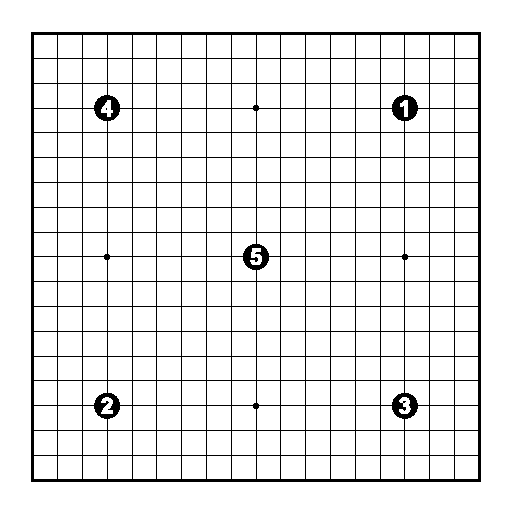
\includegraphics[width=.5\textwidth]{10 - Dia 15}
        \captionsetup{justification=centering}
        \caption*{\emph{Dia.\@~15}}
    \end{center}
    \vspace{-25pt}
\end{wrapfigure}

Quando jogadores de diferentes níveis jogam uma partida, o jogador mais forte sempre toma as pedras brancas, e a compensação é determinada pela diferença de nível entre eles. Por exemplo, se um jogador for 1 kyu, e o outro, 2 kyu, então o jogador 2 kyu não recebe nenhuma pedra de compensação. Em seu lugar, ele joga como preto sem nenhum komi, fazendo o primeiro movimento.

Quando um 1 kyu joga contra um 3 kyu, o 3 kyu recebe uma compensação de duas pedras; quando um 1 kyu joga contra um 5 kyu, o 5 kyu recebe uma compensação de quatro pedras, etc., até a compensação de nove pedras, que é em geral a maior dada.

\begin{wrapfigure}{l}{60mm}
    \vspace{-25pt}
    \begin{center}
        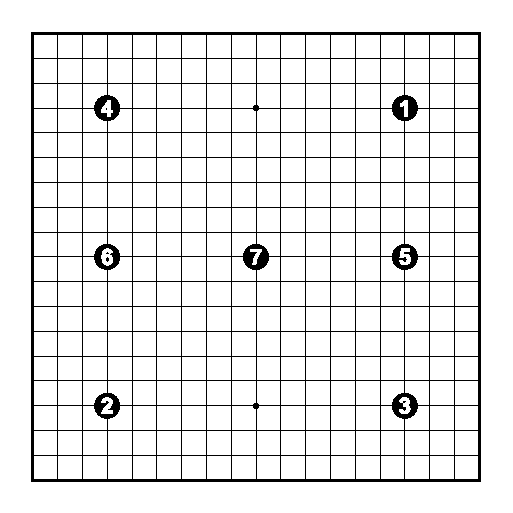
\includegraphics[width=.5\textwidth]{10 - Dia 16}
        \captionsetup{justification=centering}
        \caption*{\emph{Dia.\@~16}}
    \end{center}
    \vspace{-30pt}
\end{wrapfigure}

O mesmo sistema de compensação é utilizado para jogadores de nível dan também. A princípio, é possível determinar sua força no Go jogando contra jogadores de níveis já bem estabelecidos. No entanto, até um amador se tornar aproximadamente 5 dan, sua força pode oscilar fortemente. Por fim, apesar de que o sistema de nível do Go é virtualmente o mesmo ao redor do mundo, o valor dado a tais níveis pode variar de lugar para lugar.

\pagebreak

\begin{wrapfigure}{r}{60mm}
    \vspace{-20pt}
    \begin{center}
        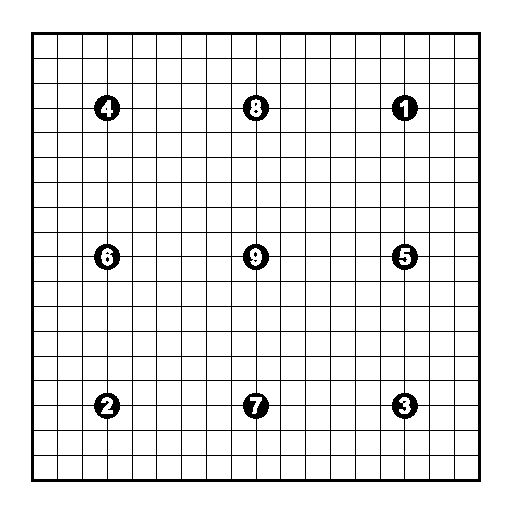
\includegraphics[width=.5\textwidth]{10 - Dia 17}
        \captionsetup{justification=centering}
        \caption*{\emph{Dia.\@~17}}
    \end{center}
    \vspace{-31pt}
\end{wrapfigure}

Assim que a compensação para o jogador mais fraco for estabelecida, ele coloca pedras de compensação no tabuleiro na ordem exibida nos \emph{Dias. 15 a 17}. Branco então faz o primeiro movimento real da partida, e ambos os jogadores se alternam. Por exemplo, se a compensação for de três pedras, Preto posicionaria as pedras 1, 2 e 3 (a ordem tradicional) no \emph{Dia.\@~15}, e Branco faria o primeiro movimento real da partida.

Seguindo estritamente as regras (\emph{Regra 4} em particular, no \autoref{chap:regras}), o que realmente está acontecendo é que, após Preto posicionar 1, Branco passa. Preto então coloca a pedra 2 (na realidade, o terceiro movimento), e, novamente, Branco passa. Preto joga 3 (movimento 4), mas Branco não passa e faz seu primeiro movimento, iniciando realmente a partida.

De acordo com a \emph{Regra 3}, um jogador pode jogar em qualquer ponto que quiser, então ele poderia jogar pedras de compensação em qualquer intersecção. É possível jogar assim\footnote{Compensação livre, em que o jogador mais fraco determina totalmente a distribuição da vantagem, é tipicamente conhecida como compensação chinesa.}, desde que negociado entre os jogadores. Porém, de um ponto de vista pedagógico, nós recomendamos seguir a maneira tradicional de se jogar Go, pois ela vai lhe ensinar como jogar com pedras no 4-4 e criar posições fortes e densas.